\appendix
\chapter{Genome preprocessing and filtering}

\begin{table}[!htp]\centering
	\scriptsize
	\begin{tabular}{cc}\toprule
		\textbf{Partition} &\textbf{Spearman Correlation} \\\midrule
		1 &0.9996 \\
		2 &0.9997 \\
		3 &0.9989 \\
		4 &0.9997 \\
		5 &0.9997 \\
		6 &0.9994 \\
		7 &0.9997 \\
		8 &0.9994 \\
		9 &0.9997 \\
		10 &0.9997 \\
		11 &0.9996 \\
		12 &0.9996 \\
		13 &0.9997 \\
		14 &0.9997 \\
		15 &0.9997 \\
		16 &0.9996 \\
		17 &0.9997 \\
		18 &0.9997 \\
		19 &0.9997 \\
		20 &0.9995 \\
		21 &0.9997 \\
		22 &0.9997 \\
		23 &0.9997 \\
		24 &0.9997 \\
		25 &0.9997 \\
		26 &0.9996 \\
		27 &0.9997 \\
		28 &0.9996 \\
		29 &0.9996 \\
		30 &0.9996 \\
		31 &0.9997 \\
		\bottomrule
	\end{tabular}
\caption[Spearman correlation assessing mean substitution effect]{Spearman correlation between corresponding partitions, comparing the cases with versus without mean substitution of missing \acp{snp}.}
\label{tab: spearman_no_vs_mean}
\end{table}

\begin{figure}[H]
	\centering
	\includesvg[width=\textwidth]{asymmetry/spearman_correlation/joinedDatasets/mean_imputed/not_subsampled/filteredSnps/filteredGwas.svg}
	\caption{Entire hemisphere \ac{gwas}, with grayed out the \acp{snp} removed when filtering with 1000G phase3 \ac{snp} set data.}
	\label{fig:1000g_entire_hemisphere}
\end{figure}

\begin{table}[H]
	\centering
	\subfloat[Overview of the entire hemisphere significant, based on the European threshold 5e-8, \ac{snp} filtering.]{
	\scriptsize
	\begin{tabular}{lcccccc}\toprule
		&\textbf{Chr.} &\textbf{\# Removed} &\textbf{\# Kept} &\textbf{Rem. Percentage} &\textbf{Removed Min. P-value} &\textbf{Kept Min. P-value} \\\midrule
		&1 &5 &1 &83.33\% &4.31e-25 &4.56e-11 \\
		&2 &175 &74 &70.28\% &1.80e-20 &4.30e-18 \\
		&3 &34 &11 &75.56\% &3.48e-15 &1.26e-15 \\
		&7 &48 &6 &88.89\% &1.76e-10 &1.13e-9 \\
		&8 &31 &16 &65.96\% &1.97e-10 &1.80e-10 \\
		&9 &28 &10 &73.68\% &1.40e-25 &1.81e-24 \\
		&12 &79 &20 &79.80\% &1.71e-13 &4.89e-13 \\
		&14 &51 &16 &76.12\% &1.09e-25 &3.58e-28 \\
		&15 &46 &9 &83.64\% &2.09e-50 &3.94e-50 \\
		&16 &467 &56 &89.29\% &3.78e-21 &1.04e-15 \\
		&17 &99 &5 &95.19\% &3.91e-44 &8.20e-31 \\
		&21 &5 &2 &71.43\% &3.01e-9 &7.89e-9 \\\midrule
		\textbf{Total} &125 &1068 &226 &82.53\% & & \\
		\bottomrule
	\end{tabular}
	\label{tab:1000g_entire_hemisphere}
}
\quad
\subfloat[Partition-chromosome pairs that had the entirety of Bonferroni significant \acp{snp} (P-value<5e-8/31) removed.]{
\scriptsize
\begin{tabular}{lccccc}\toprule
	\textbf{Chr.} &\textbf{Partition} &\textbf{\# Removed} &\textbf{Removed Min. P-value} &\textbf{Kept Min. P-value} \\\midrule
	16 &4 &6 &1.61e-11 &1.67e-8 \\
	17 &4 &40 &4.87e-11 &1.73e-8 \\
	16 &7 &3 &9.24e-16 &2.51e-9 \\
	17 &12 &4 &4.10e-10 &3.38e-9 \\
	16 &14 &4 &1.18e-13 &6.73e-9 \\
	8 &17 &1 &1.54e-9 &1.74e-9 \\
	15 &22 &1 &8.42e-10 &5.65e-9 \\
	16 &28 &2 &4.98e-10 &3.43e-8 \\
	\bottomrule
\end{tabular}
\label{tab:1000g_lost_bonf_chr}
}
\caption{Effect of 1000G Phase3 filtering on meta-analyzed \ac{gwas} scores} 

\end{table}


\begin{figure}
\begin{adjustwidth}{-3 cm}{-2.5 cm}\centering
	

	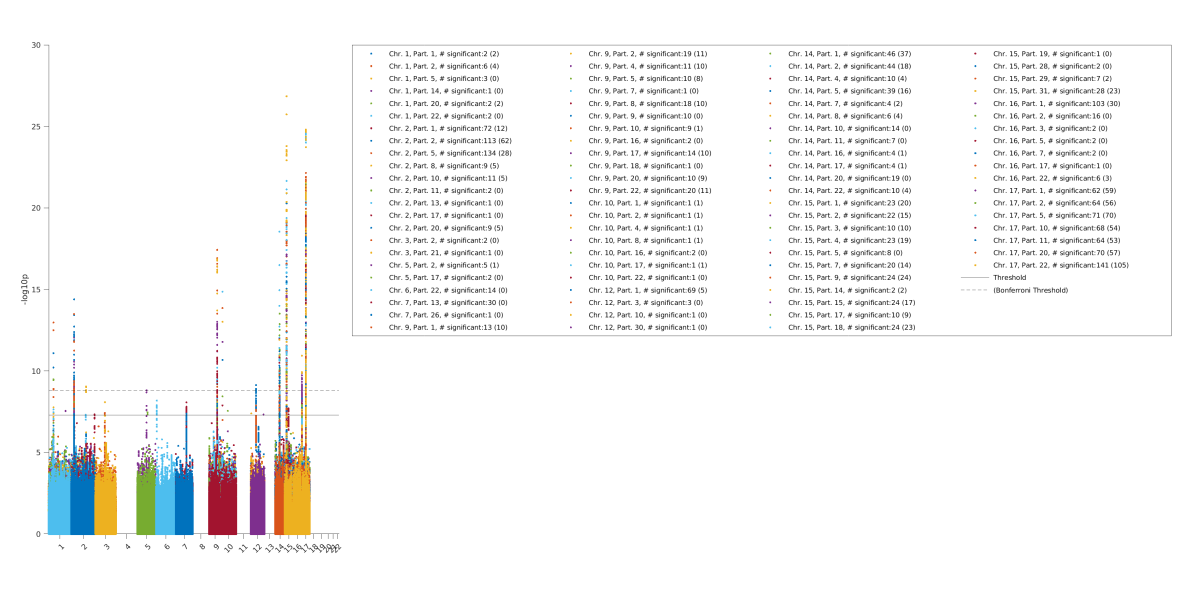
\includegraphics[width=\linewidth]{asymmetry/meta_analysis/joinedDatasets/mean_imputed/not_subsampled/partitions_gwas.pdf}
	\caption[Combined Manhattan plots across different partitions]{Combined Manhattan plots across different partitions, showing the number of significant \acp{snp} below the threshold of 5e-8 and with the Bonferroni correction, inside parentheses.}
	\label{fig:part_manhattan}


\end{adjustwidth}
\end{figure}
\chapter{Heritability}
\begin{figure}[H]
	\centering
\includesvg[width=0.5\textwidth]{asymmetry/visualizeHeritabilityOnPheno/joinedDatasets/mean_imputed/not_subsampled/Lambda GC.svg}
\caption[$\lambda_{GC}$ coefficient, as computed by LDSR]{$\lambda_{GC}$ coefficient, as computed by \ac{ldsr}. The observed $\chi^2$ value is close to the expected one at all studied partitions, with their ratio being close to 1.}	
\end{figure}
\chapter{Functional Analysis}
\begin{figure}[H]
	\centering
	\subfloat[Cell components]{
		\includegraphics[width=\textwidth]{asymmetry/FUMA gene2func/joinedDatasets/mean_imputed/not_subsampled/partitionsSummary/GO_CC.pdf}
	}
	\quad
	\subfloat[Biological processes]{
		\includegraphics[width=\textwidth]{asymmetry/FUMA gene2func/joinedDatasets/mean_imputed/not_subsampled/partitionsSummary/GO_BP.pdf}
	}
	\quad
	\subfloat[Molecular function]{
		\includegraphics[width=\textwidth]{asymmetry/FUMA gene2func/joinedDatasets/mean_imputed/not_subsampled/partitionsSummary/GO_MF.pdf}
	}
	\caption[GO terms enrichment analysis]{\Ac{go} terms enrichment analysis -log10 P-values (the higher value and the darker color, the more significant), as computed by FUMA, with the gene set augmented by GREAT.For all three cases, the entire hemisphere and the four 2nd level partition were assessed, however not all of the tests displayed a significant signal with \ac{go} terms.}
	\label{fig:go}
\end{figure}

\begin{figure}[H]
	\centering
	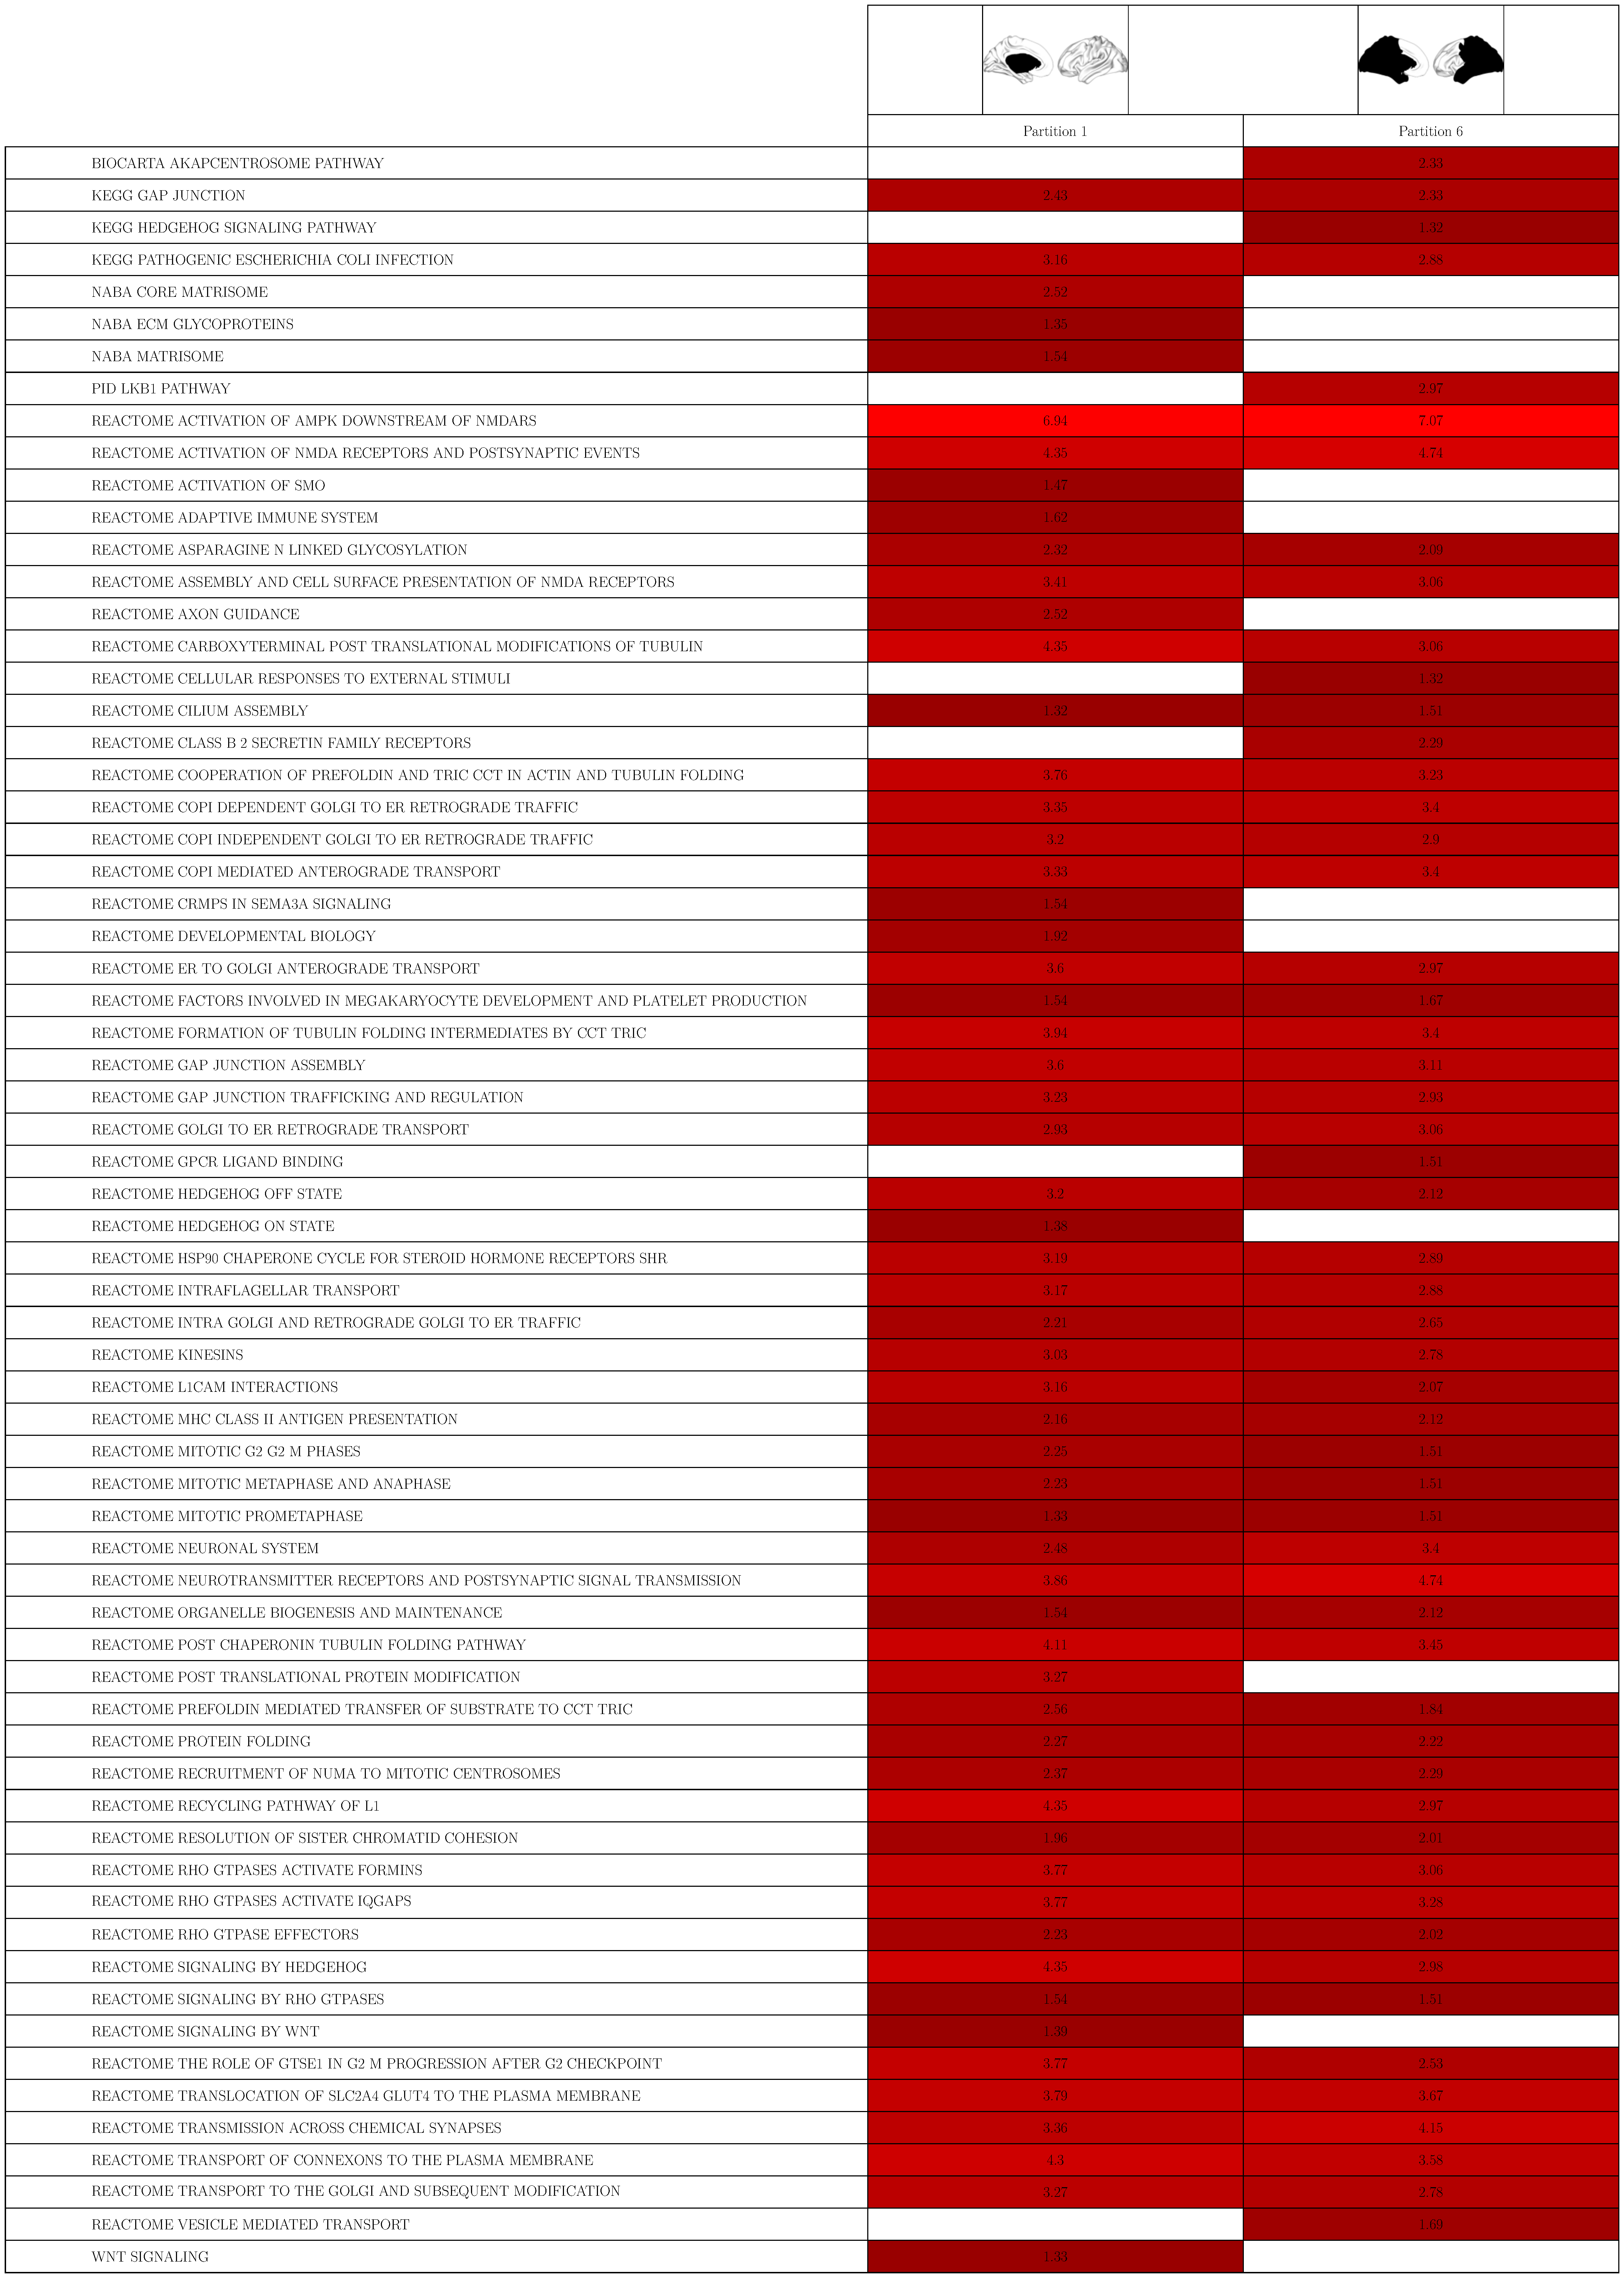
\includegraphics[width=\textwidth]{asymmetry/FUMA gene2func/joinedDatasets/mean_imputed/not_subsampled/partitionsSummary/canonical_pathways.pdf}
	
	\caption[Canonical pathways gene set enrichment analysis]{Differential gene set enrichment analysis performed on various canonical pathways reported by KEGG and Reactome, as computed by FUMA. Displayed -log10 P-values have increased lightness the higher the value.}
	\label{fig:can_pathways}
\end{figure}
\begin{figure}[H]
	\centering
	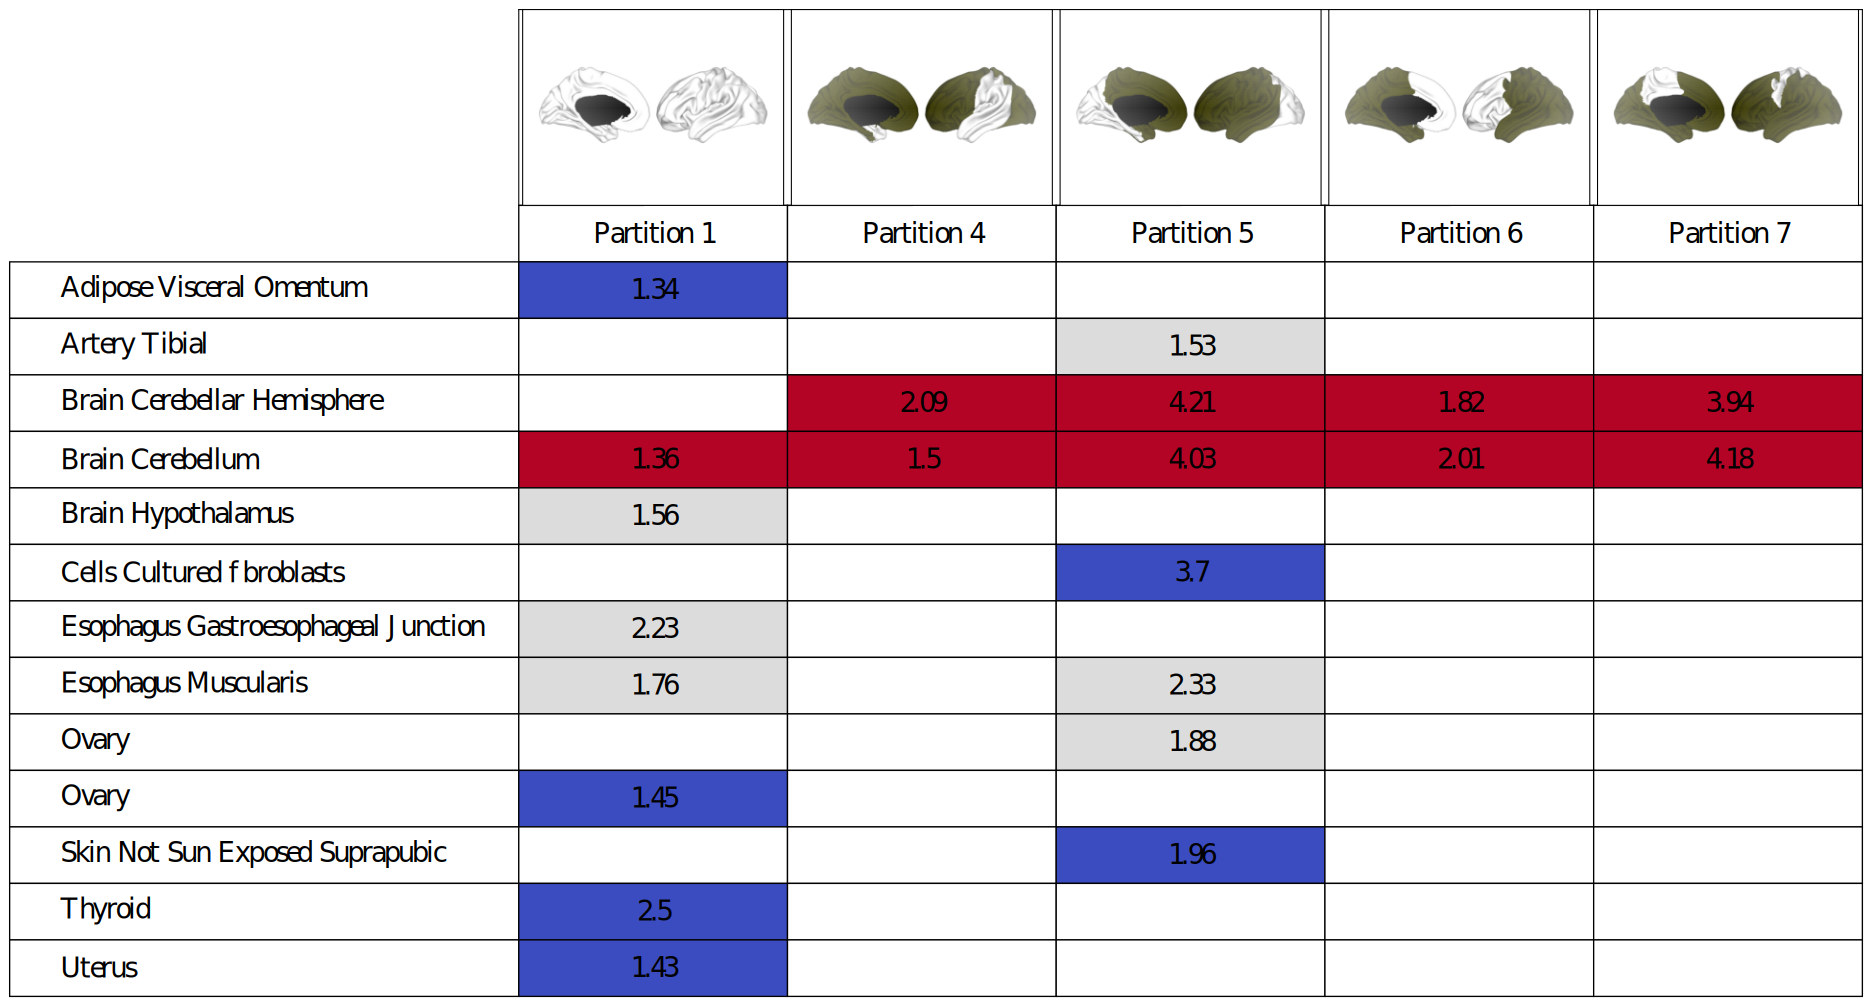
\includegraphics[width=\textwidth]{asymmetry/FUMA gene2func/joinedDatasets/mean_imputed/not_subsampled/partitionsSummary/DEG.pdf}
	
	\caption[Differential gene expression enrichment analysis]{Differential gene expression enrichment analysis performed on different tissues. Displayed -log10 P-values, as computed by FUMA using the identified partition-specific gene sets, are displayed in blue if the relation favors downregulated genes, red if it favors upregulated ones, or gray, if both downregulated and upregulated gene subsets are significantly enriched.}
	\label{fig:de_genes}
\end{figure}
\begin{figure}[H]
	\centering
	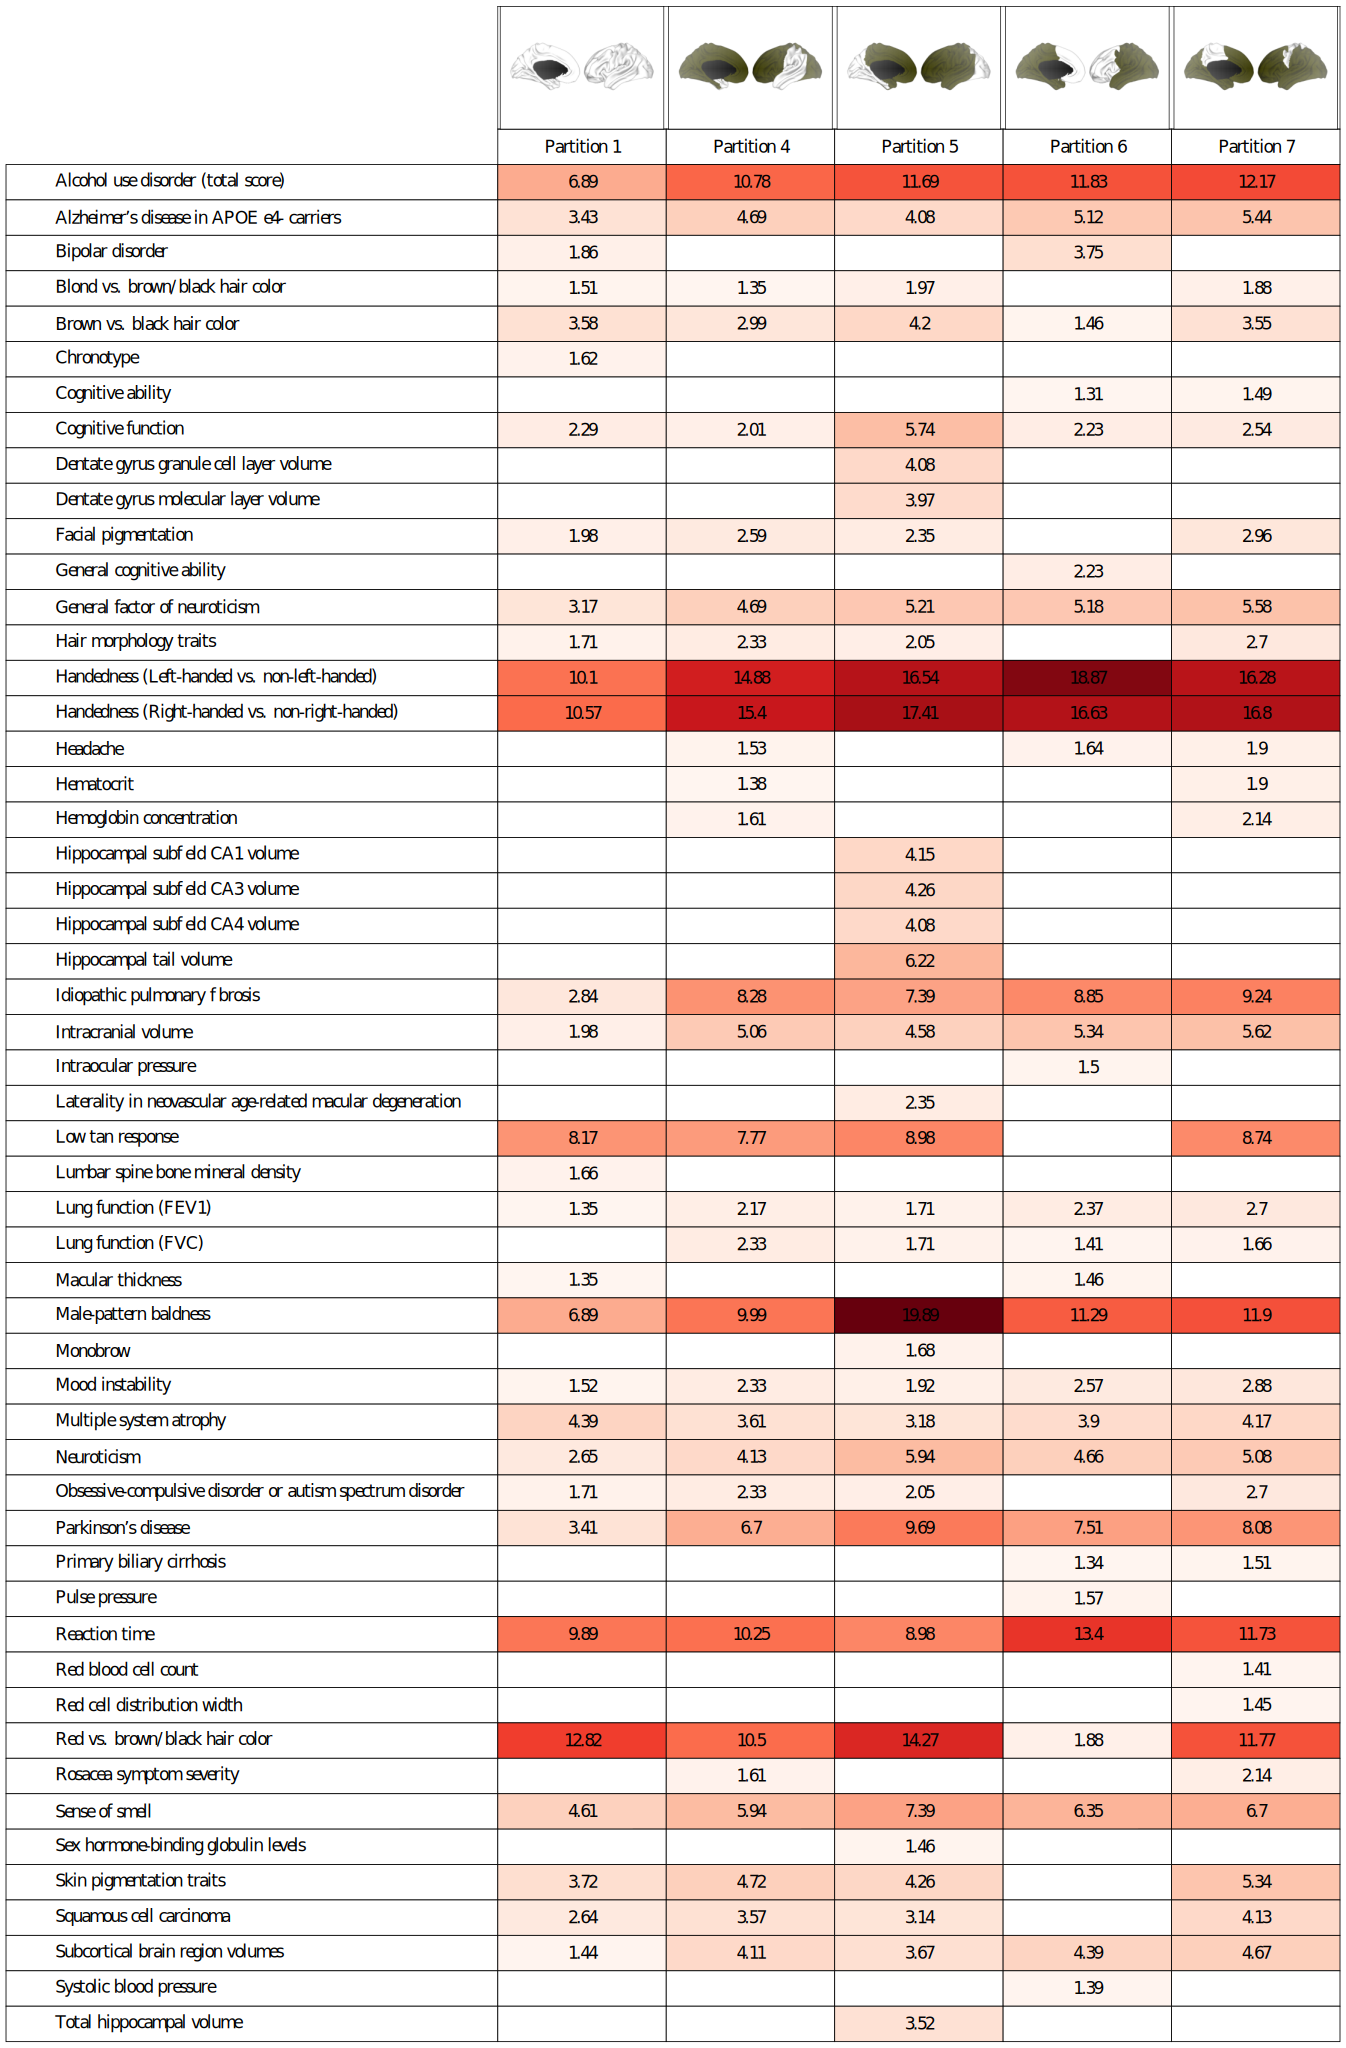
\includegraphics[width=\textwidth]{asymmetry/FUMA gene2func/joinedDatasets/mean_imputed/not_subsampled/partitionsSummary/GWASCatalog.pdf}
	
	\caption[GWAS Catalog gene set enrichment analysis]{Differential gene set enrichment analysis performed on various traits reported by GWAS catalog, as computed by FUMA. -log10 P-values are shown, with increased lightness the higher the value.}
	\label{fig:gw_catalog}
\end{figure}
